\documentclass[main]{subfiles}
\begin{document}

\section*{Lecture 20 // Oct 29 // The Casson Invariant}
\addcontentsline{toc}{section}{Lecture 20 -- The Casson Invariant}

\begin{recall}
We revisited the character variety.
\end{recall}

Today, we'll discuss the Casson invariant. For a $\mathbb{Z}\mathrm{HS}^3$ $Y$, the Casson invariant $\lambda(Y)$ is, up to a constant factor, ``the number of irreducible $\SU(2)$ representations of $\pi_1(Y)$.'' It is related to $\mathrm{IFH}_\ast$ by a famous theorem, due to Taubes:

\begin{theorem}[Taubes]
\[
\frac{1}{2}\chi\big(H_\ast(C(Y))\big) = \lambda(Y),
\]
where $\chi(H_\ast(C(Y)))$ is the Euler characteristic of the irreducible chain complex.
\end{theorem}

You might ask: isn't this tautological? Given a free, finitely generated complex, we know that the Euler characteristic of the complex is the Euler characteristic of the homology, and both objects were literally defined as a count of $\SU(2)$ representations. However, the point is that $\lambda$ is actually a completely different way to count $\SU(2)$ representations which is very classical and existed long before $\mathrm{IFH}_\ast$. We won't prove this theorem, but we will discuss its definition and a short historical overview.

What are some interesting properties of $\lambda$?
\begin{enumerate}
\item It satisfies a formula. Doing $1/n$ surgery on some $K\subset\mathbb{Z}\mathrm{HS}^3$ gives another $\mathbb{Z}\mathrm{HS}^3$, and the Casson invariants are related by
\[
\lambda\big(Y_{\frac{1}{n+1}}(K)\big) - \lambda\big(Y_{\frac{1}{n}}(K)\big) = \frac{1}{2}\Delta_K''(1),
\]
where $\Delta_K''$ is the second derivative of the Alexander polynomial evaluated at $1$. Of course, when $n=0$, $Y_{1/0}\cong Y$, and it turns out that every $\mathbb{Z}\mathrm{HS}^3$ can be obtained from $S^3$ by a sequence of $\pm 1$ surgeries on knots. This tells us that the Casson invariant is purely combinatorial (e.g., there's no gauge theory involved!), relying only on the Alexander polynomial of a knot.

\item The Casson invariant is a $\mathbb{Z}$-lift of the Rokhlin invariant:
\[
\lambda(Y) \equiv \mu(Y) \mod 2.
\]
(In fact, this is implied by (1), but we won't prove this.)
\end{enumerate}

Historically, interest in the Casson invariant was related to using the Rokhlin invariant as a possible disproof of the $3$-dimensional Poincar\'e conjecture. Before the advent of Floer/gauge theory, the hope was finding a homotopy $S^3$ with nontrivial Rokhlin invariant. But the Casson invariant says no: if you believe that the Casson invariant is a count of representations, any homotopy $S^3$ has trivial $\SU(2)$ representations, so the Rokhlin invariant is $0$.

\begin{remark}
Every $Y$ is $\pm$ surgery on a link of unknots, but $\Delta_K$ is computed at each step, so $\Delta_K\neq 1$.
\end{remark}

So what is this mysterious invariant? We said that the idea was to count conjugacy classes of $\SU(2)$ representations. How do we do this? Of course, the problem that we've seen is that the character variety $\mc{R}(Y)$ may not be discrete -- what does ``counting'' mean here? What we mean by ``count'' is an intersection number.

The idea is very geometric. Suppose $Y$ is a $\mathbb{Z}\mathrm{HS}^3$. Choose a Heegaard splitting of $Y = H_1\cup_{\Sigma_g}H_2$. We have the inclusions
\begin{center}
\begin{tikzcd}[row sep=small, column sep=large]
& H_1 \arrow[dr, hook, "j_1"] & \\
\Sigma_g \arrow[ur, hook, "\iota_1"] \arrow[dr, hook, "\iota_2"'] & & Y \\
& H_2 \arrow[ur, hook, "j_2"'] &
\end{tikzcd}
\end{center}
which induce maps on the fundamental groups
\begin{center}
\begin{tikzcd}[row sep=small, column sep=large]
& \pi_1(H_1) \arrow[dr, two heads, "j_{1\ast}"] & \\
\pi_1(\Sigma_g) \arrow[ur, two heads, "\iota_{1\ast}"] \arrow[dr, two heads, "\iota_{2\ast}"'] & & \pi_1(Y) \\
& \pi_1(H_2) \arrow[ur, two heads, "j_{2\ast}"'] &
\end{tikzcd}
\end{center}
which are clearly surjective.

Now, we introduce the following notation.

\begin{definition}
\begin{itemize}
\item The Representation Variety: $R(Y) := \mathrm{Hom}(\pi_1(Y),\SU(2))$.
\item The Irreducible Representation Variety: $R^{\mathrm{irr}}(Y) = \{\text{homomorphisms with stabilizer } \pm I\}$.
\item The Character Variety: $\mc{R}(Y) = R(Y)/\mathrm{conj}$.
\item The Irreducible Character Variety: $\mc{R}^{\mathrm{irr}}(Y) = R^{\mathrm{irr}}(Y)/\mathrm{conj}$.
\end{itemize}
\end{definition}

Applying $\mathrm{Hom}(-,\SU(2))$ to every group in the diagram reverses the arrows, giving injective maps
\begin{center}
\begin{tikzcd}[row sep=small, column sep=large]
& R(H_1) \arrow[dl, hook, "\iota_1^\ast"'] & \\
R(\Sigma) & & R(Y) \arrow[ul, hook', "j_1^\ast"'] \arrow[dl, hook', "j_2^\ast"] \\
& R(H_2) \arrow[ul, hook, "\iota_2^\ast"] &
\end{tikzcd}
\end{center}
This process preserves subgroups and is conjugation equivariant, so we could replace the ``$R$''s in the diagram with any choice of $\{R^{\mathrm{irr}}, \mc{R}, \mc{R}^{\mathrm{irr}}\}$.

What the diagram is supposed to suggest is that $\mc{R}^{\mathrm{irr}}(Y)$ can be identified with the intersection of the $H_i$'s in $\Sigma$:
\[
\mc{R}^{\mathrm{irr}}(Y) \cong (\iota_1^\ast)\mc{R}^{\mathrm{irr}}(H_1)\cap(\iota_2^\ast)\mc{R}^{\mathrm{irr}}(H_2) \quad \text{inside } \mc{R}^{\mathrm{irr}}(\Sigma)
\]

This makes sense, since every representation on $\pi_1(Y)$ must split into representations on $\pi_1(H_1)$ and $\pi_1(H_2)$ which agree over their intersection, so the representation on $\pi_1(Y)$ should be determined by the representation on $\pi_1(\Sigma)$. This is good because these are very simple!

\begin{proposition}
$\mc{R}^{\mathrm{irr}}(H_1)$ is an open manifold of dimension $3g-3$.
\end{proposition}

\begin{proof}
First note that since $\pi_1(H_1)\cong \ast_g\mathbb{Z}$, $R(H_1) = \SU(2)^g$ -- though $\mc{R}^{\mathrm{irr}}\subset\mc{R}$ is complicated. Therefore
\[
\dim(\mc{R}^{\mathrm{irr}}(H_1)) = \dim(\SU(2)^g) - \dim(\text{conj action}) = 3g - \dim(\SU(2)) = 3g-3.
\]
Being irreducible is a closed condition, so $\mc{R}^{\mathrm{irr}}$ is open. \qedhere
\end{proof}

\begin{proposition}
$\mc{R}^{\mathrm{irr}}(\Sigma)$ is an open manifold of dimension $6g-6$.
\end{proposition}

\begin{proof}
Recall that $\pi_1(\Sigma_g) = \langle a_1,b_1,\dots,a_g,b_g \mid \prod[a_i,b_i]=1\rangle$, which we can interpret as $f^{-1}(1)$ for the map
\[
f : \mathop{\ast}_{2g}\mathbb{Z}\longrightarrow\mathbb{Z}, \qquad (a_1,b_1,\dots,a_g,b_g)\longmapsto\prod[a_i,b_i].
\]
For any representation, this gives a map
\[
f_\rho : \SU(2)^{2g}\to\SU(2), \qquad (A_1,B_1,\dots,A_g,B_g)\longmapsto\prod[A_i,B_i],
\]
so $\rho(\pi_1(\Sigma)) = f_\rho^{-1}(I)$. It turns out that $Df$ is surjective for irreducible representations, so
\[
\dim(\mc{R}^{\mathrm{irr}}(\Sigma)) = 6g-3-\dim(\SU(2)) = 6g-6.
\]
Similarly, being reducible is a closed condition, so $\mc{R}^{\mathrm{irr}}(\Sigma)$ is open. \qedhere
\end{proof}

\begin{definition}
Choose a compactly supported perturbation (or isotopy) of $\mc{R}^{\mathrm{irr}}(H_2)$ inside $\mc{R}(\Sigma)$ such that
\[
(\iota_1^\ast)\mc{R}^{\mathrm{irr}}(H_1)\pitchfork(\iota_2^\ast)\mc{R}^{\mathrm{irr}}(H_2).
\]
The Casson invariant is
\[
\lambda(Y) = \left(\frac{(-1)^g}{2}\right)\cdot\left(\begin{array}{c}\text{Signed number of intersections between} \\ (\iota_1^\ast)\mc{R}^{\mathrm{irr}}(H_1) \text{ and the perturbed } (\iota_2^\ast)\mc{R}^{\mathrm{irr}}(H_2)\end{array}\right).
\]
\end{definition}

This definition begs a few questions! It turns out that the representation varieties can be oriented, so we can take a signed count of intersections. The factor of $(-1)^g$ is to account for different choices of Heegaard splittings, though why the signed count is divisible by $2$ is not obvious.

However, you should ask: what's up with needing a compactly supported perturbation? The point here is that $\mc{R}(\Sigma)$ is not a smooth manifold! It contains a singular locus of reducible representations, which we must avoid when performing our signed count since the ambient space is not a manifold. This introduces some complexities.
\begin{center}
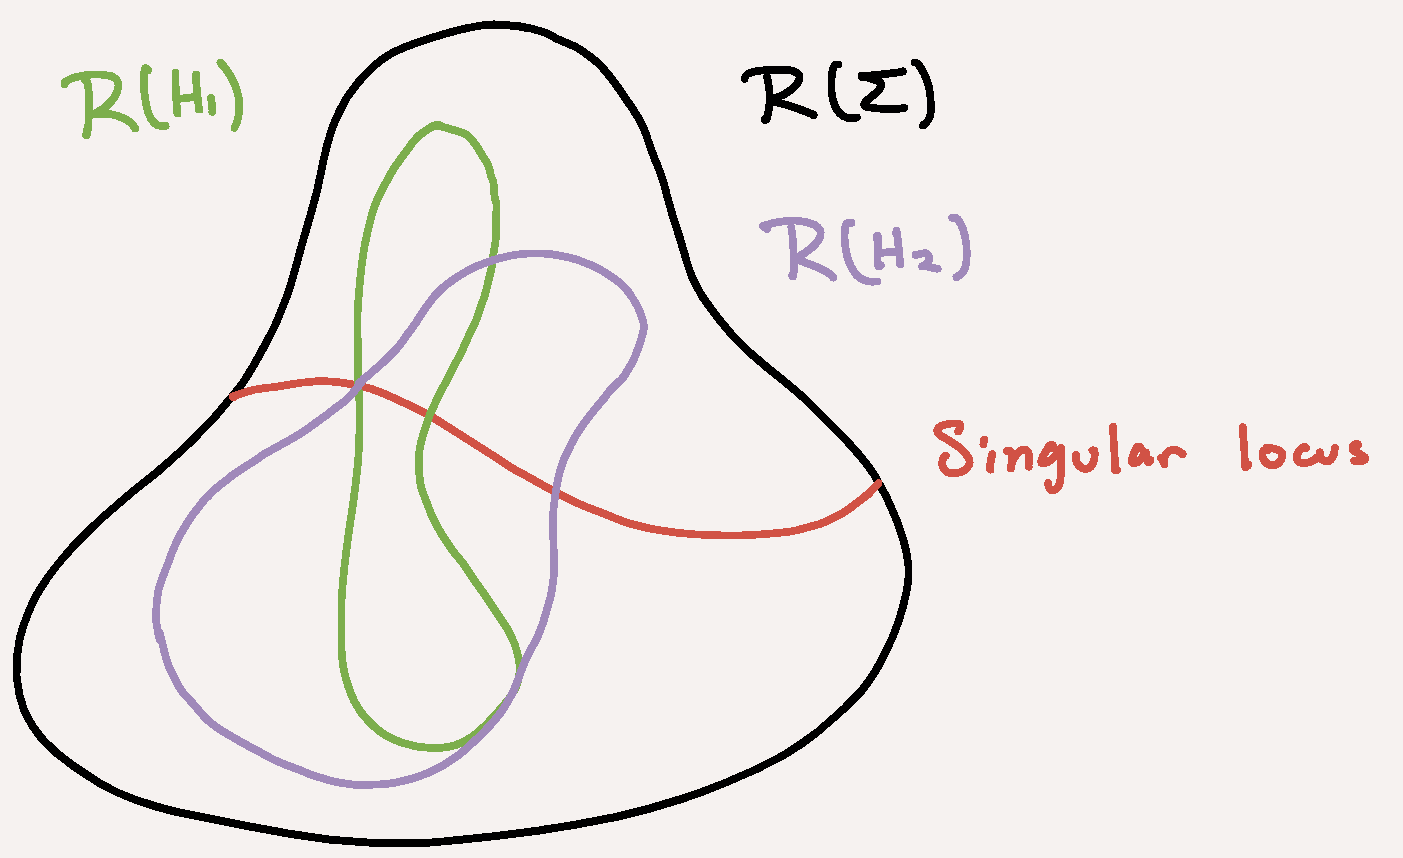
\includegraphics[width=0.45\linewidth]{figures/fig_lec20_rep_sigma.png}
\end{center}

We need to perturb in the first place to ensure transversality. If these perturbations can be supported everywhere, who's to say we can't perturb every intersection away! Also, we must take our perturbation to be away from the singular locus. In other words, if the perturbation isn't compactly supported, it need not fix the endpoints of $\mc{R}(H_2)\cap$ open ball. The local picture is:
\begin{center}
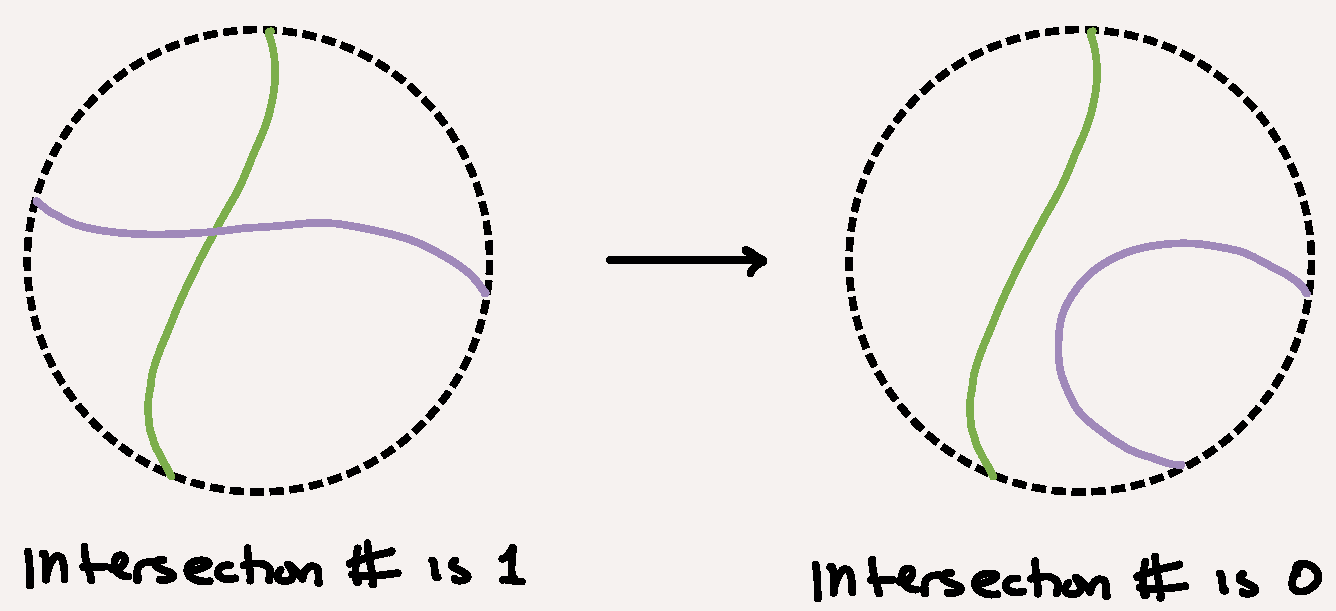
\includegraphics[width=0.85\linewidth]{figures/fig_lec20_local_perturb.png}
\end{center}

The one caveat is that restricting the type of perturbation restricts the type of intersections we can perturb away! That is, if the intersection set itself is not compact, we're stuck. This means that the set is open -- so they intersect in the singular locus as well.

Given that $\mc{R}(H_1)$ and $\mc{R}(H_2)$ intersect at a reducible representation, let's consider what they could look like nearby:
\begin{center}
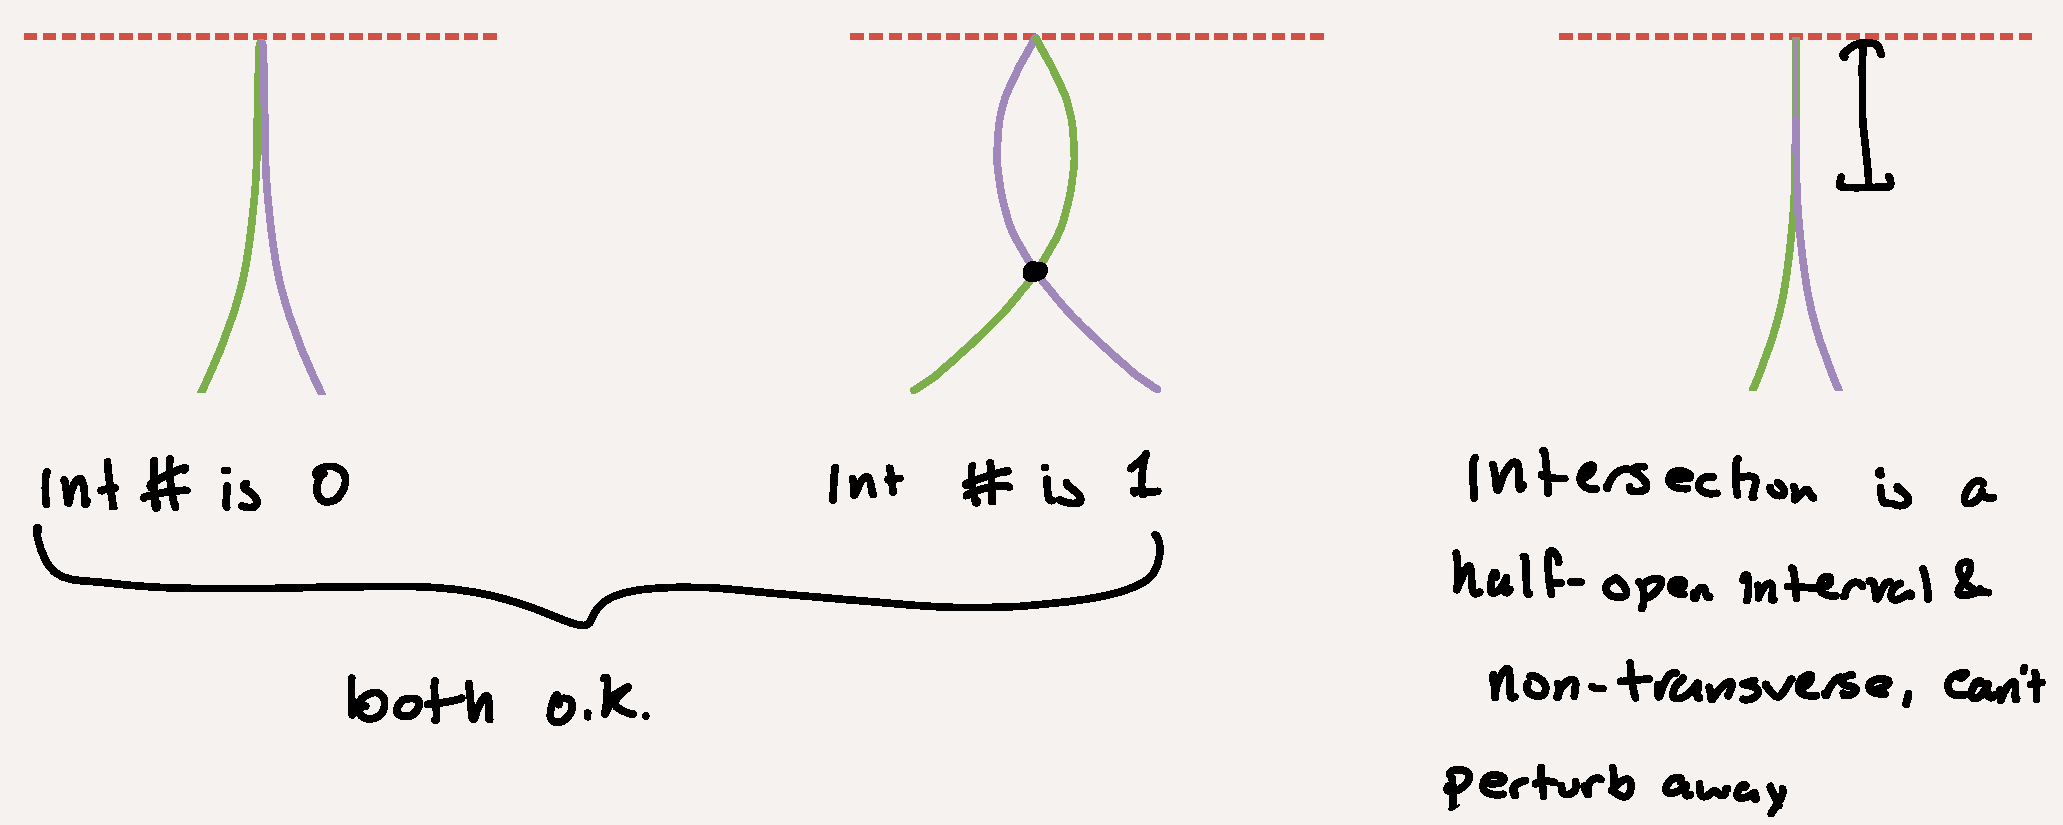
\includegraphics[width=0.75\linewidth]{figures/fig_lec20_reducible_cases.png}
\end{center}

% NOTE: this was originally a claim environment (changed to proposition)
\begin{proposition}
The third case can't happen.
\end{proposition}
The point here is that we need to prove some analytic properties to make sense of the intersection number, since we're not working in a smooth manifold.

\begin{proposition}
For a $\mathbb{Z}\mathrm{HS}^3$, $\mc{R}(H_1)$ and $\mc{R}(H_2)$ intersect in the singular locus in exactly one point.
\end{proposition}

\begin{proof}
Consider the trivial representations of $\pi_1(H_1)$ and $\pi_1(H_2)$; clearly they both restrict to the trivial representation of $\pi_1(\Sigma)$, so they are an element of $\mc{R}(Y)$. Since the identity is stabilized by the entire group, it is in the singular locus. Any other representation in this locus must have nontrivial stabilizer, so it must be abelian. Thus the representation factors through $\pi_1^{\mathrm{ab}}(Y)=H_1(Y)=0$ since $Y$ is a $\mathbb{Z}\mathrm{HS}^3$. \qedhere
\end{proof}

However, recall from last time that we claimed that for the $n=3$ Brieskorn spheres the set of points was an honest count without perturbation. This means that $\mc{R}(H_1)$ and $\mc{R}(H_2)$ can't intersect non-transversely, even if the intersection is discrete:
\begin{center}
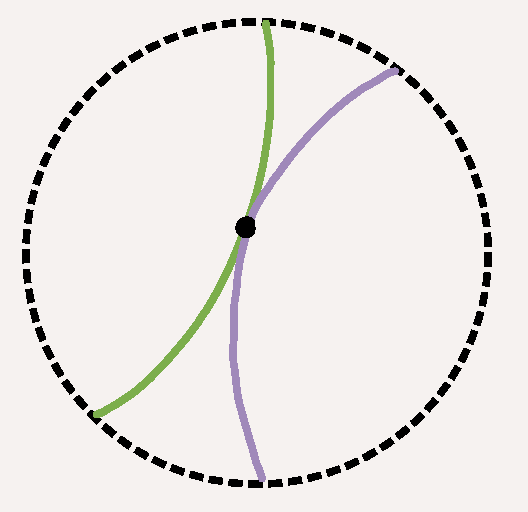
\includegraphics[width=0.25\linewidth]{figures/fig_lec20_tangent_int.png}
\end{center}

\begin{proposition}
For the $n=3$ Brieskorn sphere, the ``naive'' point count is the count as for $\lambda$.
\end{proposition}

But how can we even verify this? Or, what even are the tangent spaces, explicitly? How do we calculate their intersection? In order to discuss transversality, it will be convenient to introduce some language from algebraic geometry.

\subsection*{Interlude}

Let $\pi$ be a finitely presented group, thought of as $\pi=\pi_1(X)$. Let $\rho:\pi\to\SU(2)$ be a representation.

What is $T_\rho R(\pi)$, i.e., the tangent space to the representation variety at the representation $\rho$? If we forget, for a second, that $\rho$ is a group homomorphism, $\rho$ is just some map from $\pi$ to $\SU(2)$. Given $\rho\in\mathrm{Map}(\pi,\SU(2))$, we can ask the more general question: what is $T_\rho\mathrm{Map}(\pi,\SU(2))$?

A tangent space at a point can be thought of as the space of directions you can move (perturb) in to stay in whichever locus the point is in. Explicitly, for some $x\in\pi_1$, a ``nearby'' map to $\rho(x)$ is of the form $\rho(x)+\epsilon\beta(x)$, for $\beta(x)\in T_{\rho(x)}\SU(2)$.
\begin{center}
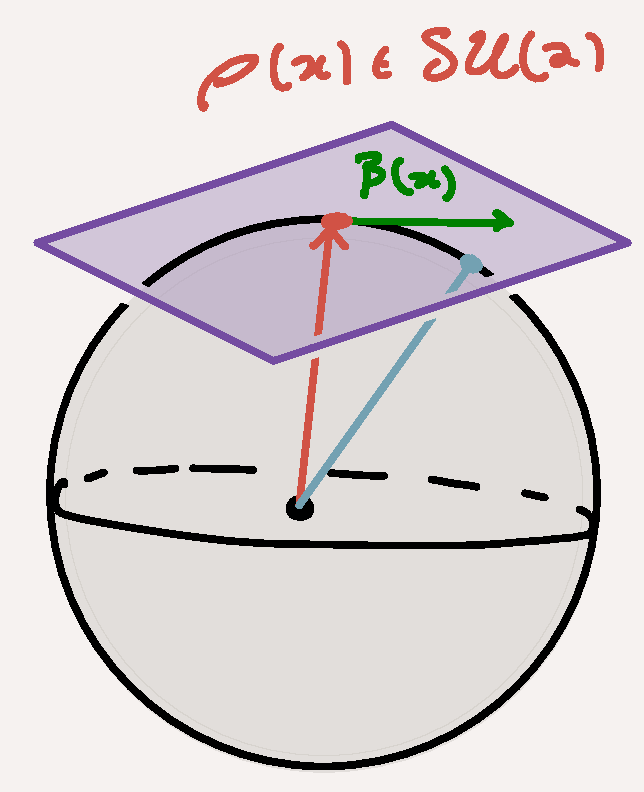
\includegraphics[width=0.3\linewidth]{figures/fig_lec20_tangent_su2.png}
\end{center}
But it's more convenient to remember that right multiplication moves $T_1\SU(2)$ to $T_{\rho(x)}\SU(2)$, so we can think of $\beta(x)\in T_{\rho(x)}\SU(2)$ instead as $\beta(x)=\eta(x)\rho(x)$, for $\eta(x)\in T_1\SU(2)=\mathfrak{su}(2)$. Therefore the new point is
\[
\rho(x)+\epsilon\beta(x) = \rho(x)+\epsilon\eta(x)\rho(x) = (1+\epsilon\eta(x))\rho(x).
\]

Now we have an explicit understanding of what it means to be in $T_\rho\mathrm{Map}(\pi,\SU(2))$. But not every map is a representation. So we must ask which maps are homomorphisms, at least to $1^{\text{st}}$ order. Let's linearize the condition $\rho(xy)=\rho(x)\rho(y)$.

For a perturbation $\eta(x):\pi\to\mathfrak{su}(2)$, we need $\rho(xy)+\epsilon\eta(xy)\rho(xy)$ to equal (up to first order)
\[
\big(\rho(x)+\rho(x)\epsilon\eta(x)\big)\big(\rho(y)+\rho(y)\epsilon\eta(y)\big).
\]
Expanding,
\[
\big(\rho(x)+\rho(x)\epsilon\eta(x)\big)\big(\rho(y)+\rho(y)\epsilon\eta(y)\big) = \rho(x)\rho(y)+\rho(x)\epsilon\eta(x)\rho(y)+\rho(x)\rho(y)\epsilon\eta(y) + \underbrace{\rho(x)\epsilon\eta(x)\rho(y)\epsilon\eta(y)}_{2^{\text{nd}}\text{ order}}.
\]
So if $\rho(xy)+\epsilon\eta(xy)\rho(xy) = \rho(x)\rho(y)+\rho(x)\epsilon\eta(x)\rho(y)+\rho(x)\rho(y)\epsilon\eta(y)$, and if we know $\rho(xy)=\rho(x)\rho(y)$, $\rho(x)\eta(x)=\eta(x)\rho(x)$, $\rho(y)\eta(y)=\eta(y)\rho(y)$, then
\begin{align*}
\epsilon\eta(xy)\rho(xy) &= \rho(x)\epsilon\eta(x)\rho(y)+\rho(x)\rho(y)\epsilon\eta(y)\\
\eta(xy)\rho(x)\rho(y) &= \rho(x)\eta(x)\rho(y)+\rho(x)\rho(y)\eta(y)\\
\eta(xy) &= \rho(x)\eta(x)\rho(y)\rho(y)^{-1}\rho(x)^{-1}+\rho(x)\rho(y)\eta(y)\rho(y)^{-1}\rho(x)^{-1}\\
\eta(xy) &= \eta(x)+\rho(x)\eta(y)\rho(x)^{-1}.
\end{align*}
Setting $\mathrm{Ad}_{\rho(x)}\eta(y) := \rho(x)\eta(y)\rho(x)^{-1}$, we can conclude that
\[
\eta(xy) = \eta(x)+\mathrm{Ad}_{\rho(x)}\eta(y).
\]
This gives an ``algebraists'' explicit description of the tangent space of a representation in representation space.

\begin{definition}
The Zariski tangent space is
\[
Z^1_\rho = \left\{\eta:\pi\to\mathfrak{su}(2) \,\Big|\, \eta(xy)=\eta(x)+\mathrm{Ad}_{\rho(x)}\eta(y)\right\}.
\]
\end{definition}

This is a generalized notion of tangent space which is defined at singular points, but if $\rho$ is a smooth point of $R(\pi)$, then $Z^1_\rho$ is the tangent space, so this recovers the usual notion of the tangent space.

\begin{remark}
$Z$ doesn't stand for Zariski, and the $1$ doesn't mean $1^{\text{st}}$ order\dots the reason for this notation will soon become clear.
\end{remark}

Now, we wish for a definition of the tangent space in the character variety. We get $\mc{R}$ from $R$ by quotienting by the $\SU(2)$ action, so let's try to quotient $Z^1_\rho$ by this action as well. What is
\[
T_\rho\left(\begin{array}{c}\text{orbit of } \rho \text{ under} \\ \text{conj action}\end{array}\right)?
\]
\begin{center}
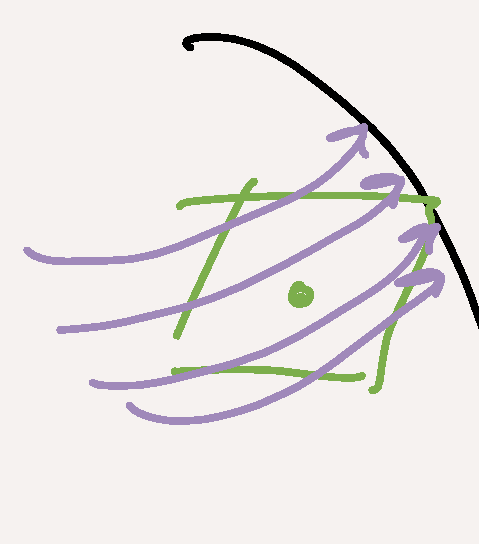
\includegraphics[width=0.2\linewidth]{figures/fig_lec20_orbit.png}
\end{center}
Fix $u\in\mathfrak{su}(2)$. Conjugating $\rho$ by an element which is very close to the identity sends $\rho$ to $(1+\epsilon u)\rho(1-\epsilon u)$. Expanding,
\[
(1+\epsilon u)\rho(1-\epsilon u) = \rho+\epsilon u\rho-\rho\epsilon u = \big(1+\epsilon(u-\mathrm{Ad}_\rho u)\big)\rho.
\]
So when we act by a small gauge transformation, the direction $\rho$ moves along is $\mathrm{Ad}_\rho u=\rho(x)u\rho(x)^{-1}$.

\begin{definition}
\[
B^1_\rho = \left\{\eta:\pi\to\mathfrak{su}(2) \,\Big|\, \exists\, u\in\mathfrak{su}(2) \text{ such that } \eta(x) = u-\mathrm{Ad}_{\rho(x)}u\ \ \forall x\right\}.
\]
\end{definition}

Putting this all together, we have discovered that
\[
T_{[\rho]}\mc{R}(\pi) = Z^1_\rho/B^1_\rho.
\]

\begin{definition}
The $1^{\text{st}}$ group cohomology of $\pi$ is
\[
H^1_\rho(\pi,\mathfrak{su}(2)) = Z^1_\rho/B^1_\rho = T_{[\rho]}\mc{R}(\pi).
\]
Explicitly, what we mean is the $1^{\text{st}}$ group cohomology with elements in $\mathfrak{su}(2)$, twisted by $\rho$.
\end{definition}

\begin{remark}
So $Z$ and $B$ are cocycles and coboundaries and $1$ is $1^{\text{st}}$!
\end{remark}

By construction, $\dim(T_{[\rho]}\mc{R}(\pi))$ is the expected dimension of the representation space at that representation.

Back to earth: how does this relate to the character variety?

\begin{lemma}
Let $\rho$ be an irreducible representation coming from $\mc{R}^{\mathrm{irr}}(H_1)\cap\mc{R}^{\mathrm{irr}}(H_2)$, where $\mc{R}^{\mathrm{irr}}(H_2)$ is not perturbed. This intersection is transverse at $\rho$ if and only if $H^1_\rho(\pi,\mathfrak{su}(2))=0$.
\end{lemma}

\begin{proof}
We do some slight abstract nonsense: there is a long exact sequence for group cohomology:
\[
H^0_\rho(\pi_1(\Sigma),\mathfrak{su}(2))\to H^1_\rho(\pi_1(Y),\mathfrak{su}(2))\to
\]
\[
H^1_\rho(\pi_1(H_1),\mathfrak{su}(2))\oplus H^1_\rho(\pi_1(H_2),\mathfrak{su}(2))\xrightarrow{\ \iota_1^\ast\oplus\iota_2^\ast\ }H^1_\rho(\pi_1(\Sigma),\mathfrak{su}(2)).
\]
The transversality condition is precisely that the map $\iota_1^\ast\oplus\iota_2^\ast$ is surjective. At a smooth point, we asserted that this construction was the same as the normal tangent space, so $\dim(H^1_\rho(\pi_1(H_i),\mathfrak{su}(2)))=3g-3$ and $\dim(H^1_\rho(\pi_1(\Sigma),\mathfrak{su}(2)))=6g-6$. Therefore $\iota_1^\ast\oplus\iota_2^\ast$ is surjective if and only if it is an isomorphism.

We haven't yet defined the $0^{\text{th}}$ group cohomology:
\[
H^0_\rho(\pi_1(\Sigma),\mathfrak{su}(2)) = \left\{u\in\mathfrak{su}(2) \,\Big|\, u-\mathrm{Ad}_{\rho(x)}u=0\ \ \forall x\right\},
\]
which is nonzero if there exists an infinitesimal conjugation which doesn't move the representation. If there existed such a $u$, it would have nontrivial stabilizer -- but we're only working with irreducibles, so
\[
H^0_\rho(\pi_1(\Sigma),\mathfrak{su}(2))=0.
\]
Therefore $\iota_1^\ast\oplus\iota_2^\ast$ is an isomorphism. \qedhere
\end{proof}

The moral here is that to know whether we must perturb, it is enough to check if $H^0_\rho(\pi_1(\Sigma),\mathfrak{su}(2))=0$.

\end{document}
